\section{Praktikos veiklos aprašymas}
Šį skyrių sudaro praktikos veiklos aprašymas ir jos įgyvendinimas.

\subsection{Praktikos vietos gavimas}
Norint gauti praktikos vietą \enquote{Bentley systems} reikėjo atlikti 3 su programavimu susijusias užduotis \enquote{Codility} aplinkoje. Jei šios užduotys buvo atliktos gerai, kandidatas kviečiamas antram etapui. Antrojo etapo metu \enquote{Codility} aplinkoje susipažinama su programuotojais, kurie stebės kandidato užduočių atlikimą, padės jei iškils problemų. Prieš pradedant atlikti naujas užduotis, diskutuojamos pirmo etapo užduotys, kas galėjo būti geriau, kodėl tam tikri kodo sprendimai buvo priimti. Po diskusijos pateikiamos pora užduočių, kandidatas bando jas išspręsti, užstrigus, programuotojai padeda. Užduotys olimpiadinio programavimo pobūdžio ir objektinio programavimo pagrindų patikrinimo.

Pirmoji darbo diena prasidėjo nuo terminuotos sutarties pasirašymo. Po to supažindino su komanda, mentoriumi, su kuriuo dirbsiu artimiausius 3 mėnesius. Komandą sudaro 15 narių: 3 testuotojai, 1 projektų vadovas ir 12 įvairaus lygio programuotojų. Kas 3 savaites susitinkama su mentoriumi pasidalinti su per 3 savaites įvykusiais įvykiais, atsiradusiomis problemomis, diskutuojama kaip jos galėtų būti išspręstos.

% Praktikos veiklos aprašymas (vienas arba keli skyriai). Aprašomas praktikos užduoties įgyvendinimas (pvz., atlikti projektavimo ir/ar programavimo darbai, sukurtas modelis, priimti sprendimai ir pan.).
\subsection{Praktikos užduotys}

Šiame poskyryje pateiktos visos užduotys, kurios buvo atliktos praktikos metu. Kiekviena užduotis bus trumpai apibūdinta, įvardinant jos tikslą, naudotus metodus ir pasiektus rezultatus.
Reikalavimai atliekant užduotį:

\subsubsection{Tap to fullscreen on iOS}

Ši užduotis buvo skirta realizuoti programos lango pakeitimą į pilno ekrano režimą spustelėjus ant tuščios dokumente vietos, Pdf peržiūros lange. Užduotis buvo paskirstyta į 2 dalis: Android ir iOS. Pasirinkau realizuoti funkcionalumą iOS prietaisuose.

Reikalavimai atliekant užduotį:

\begin{enumerate}
    \item PdfTron anotacijų sąrašas:
    \begin{enumerate}
        \item Komponentų paslėpimas: \enquote{PdfTron}, \enquote{Synchro field} navigacijos, statuso juosta ir apatinė anotacijų juosta turėtų būti paslėpti, kai pdf ekranas apima visą ekraną.
        \item Pdf užimti visą ekraną ir sugrįžti atgal į normalią būseną.
    \end{enumerate}
    \item Kai anotacijų sąrašas atidarytas(telefone):
    \begin{enumerate}
        \item Turėtų elgtis taip pat, tik anotacijų sąrašas turi irgi dingti, kai Pdf ekranas užima visą ekraną.
    \end{enumerate}
    \item Kai anotacijų sąrašas atidarytas(plančetiniame):
    \begin{enumerate}
        \item Turėtų elgtis taip pat, tik šoninio anotacijų sąrašo neuždaryti.
    \end{enumerate}
\end{enumerate}


\enquote{Synchro Field} projekte norint peržiūrėti Pdf failus naudojame biblioteką \enquote{PdfTron} (\ref{fig:pdfViewController screen} paveikslėlis). Tačiau, \enquote{PdfTron} komponento navigacijos juosta yra atskirta nuo \enquote{Synchro field} navigacijos juostos (\ref{img:pdfViewController} paveikslėlis). Reikėjo pridėti pakeitimus funkcijai, kuri įvykdoma, kai \enquote{PdfTron} navigacijos juostos matomumas pasikeičia. \ref{fig:pdfTronCode} paveikslėlyje galime matyti, kad funkcijai pradėjus vykdymą, naudojama \textit{UIView.animate()} funkcija, kuri sklandžiai suanimuoja vartotojo sąsajos pasikeitimus. Patikrinama ar naujas funkcionalumas yra įjungtas su \enquote{feature flag}. Atliekami \enquote{Synchro field} navigacijos juostos apribojimų reikšmių pakeitimai. Animacijos trukmė parinkta 0,2 sekundės, siekiant sulyginti \enquote{PdfTron} ir \enquote{Synchro field} navigacijos laukų animacijų trukmes. Jei anotacijų sąrašas yra atidarytas (\ref{img:annotationList} paveikslėlis), sąrašas paslepiamas.

Šio funkcionalumo programavimo metu teko ne tik rašyti kodą, bet ir išmokti naudotis \enquote{Storyboards}. \enquote{PdfTron} lange reikėjo pridėti papildomų apribojimų (\emph{angl. constraints}), siekiant padidinti Pdf komponento dydį.


\begin{figure}[htbp!]
    \centering
\begin{minted}[linenos,tabsize=1,breaklines]{swift}
extension PdfTronViewController: PdfTronNavigationControllerDelegate {
    func pdfTronNavigationController(didSetNavigationBarHidden isHidden: Bool) {
        UIView.animate(withDuration: 0.2) { [weak self] in
            guard let self else { return }
            if Features.isEnabled(DevelopmentFeatureFlag.pdfMarkupNative) {
                labeledBottomBarHeightConstraint.isActive = isHidden
            }
            setNavigationBarVisibility(isHidden)
            view.layoutIfNeeded()
        }

        if let resizablePanelViewController, resizablePanelViewController.panelStatus != .closed {
            resizablePanelViewController.shouldResize = !isHidden
            let panelHeight = isHidden ? 0 : resizablePanelViewController.heightHalfExpanded
            resizablePanelViewController.animatePanelToHeight(panelHeight)
        }
    }

    private func setNavigationBarVisibility(_ isHidden: Bool) {
        setStatusBarHidden(isHidden)
        if Features.isEnabled(DevelopmentFeatureFlag.pdfMarkupNative) {
            navigationBarTopConstraint.isActive = isHidden
            navigationBarSafeAreaTopConstraint.isActive = !isHidden
            navigationBarShowingConstraint.constant = isHidden ? 0 : navigationBarHeight
        }
    }
}
\end{minted}
\caption{PdfTronViewController matomumo kodas}
    \label{fig:pdfTronCode}
\end{figure}


    
\subsubsection{UIButton configuration}
Ši užduotis buvo skirta perkelti didžiąją dalį mygtukų iOS projekte į FieldUIComponents projektą ir su vienodinti stilių nustatymą naudojant \enquote{UIButton.Configuration}.

Reikalavimai atliekant užduotį:
\begin{enumerate}
    \item Perkelti mygtuko vartotojo sąsajos kodą į FieldUIComponents projektą.
    \item Atnaujinti Field projekto kodo bazę su naujais mygtukų komponentais.
    \item Vizualių pakeitimų neturi būti.
\end{enumerate}

Pirmiausia buvo pereita per visą projektą, pažymėtos vietos, klasių mygtukai, kurie galėtų būti perkelti į FieldUIComponents projektą. Perkėlus mygtukus, pradėta perrašyti mygtukų stiliaus nustatymas su \enquote{UIButton.Configuration} (\ref{fig:Primary button} paveikslėlis). Teksto spalvos, šrifto ir dydžio nustatymas negalėjo būti perrašytas \enquote{UIButton.Configuration} pagalba, nes pakeitus mygtuko tekstą, reikšmės įgavo pradines stiliaus reikšmes. 

\begin{figure}[htbp!]
    \centering
    \begin{minted}[linenos,tabsize=1,breaklines]{swift}
@IBDesignable public class PrimaryButton: BaseUIButton {
    override func sharedInit() {
        var configuration = UIButton.Configuration.plain()
        configuration.background.cornerRadius = 3
        configuration.background.backgroundColor = UIColor(fieldColor: .blueCerulean)
        configuration.titleLineBreakMode = .byTruncatingMiddle
        self.configuration = configuration
        setAttributedTitle(font: UIFont.openSans(ofSize: 14), foregroundColor: UIColor(fieldColor: .white))
    }
    ...
}
    \end{minted}
    \caption{Primary button kodo perrašymas naudojant UIButton.Configuration}
    \label{fig:Primary button}
\end{figure}


Taip pat buvo sukurtas FieldUIComponentsApp langas, kuriame galima rasti visus projekte naudojamus mygtukus (\ref{fig:buttonsView.png} paveikslėlis). Kadangi mygtukų langas parašytas su SwiftUI, o patys mygtukai su UIKit funckijomis, reikėjo sukurti\textit{ButtonViewRepresentable}, kuris pasirinktą UIView komponento klasė supakuojama į SwiftUI komponentą, realizavus \textit{UIViewRepresentable} klasės funkcijas (\ref{fig:buttonViewRepresentable} paveikslėlis).

\begin{figure} [htbp!]
    \centering
    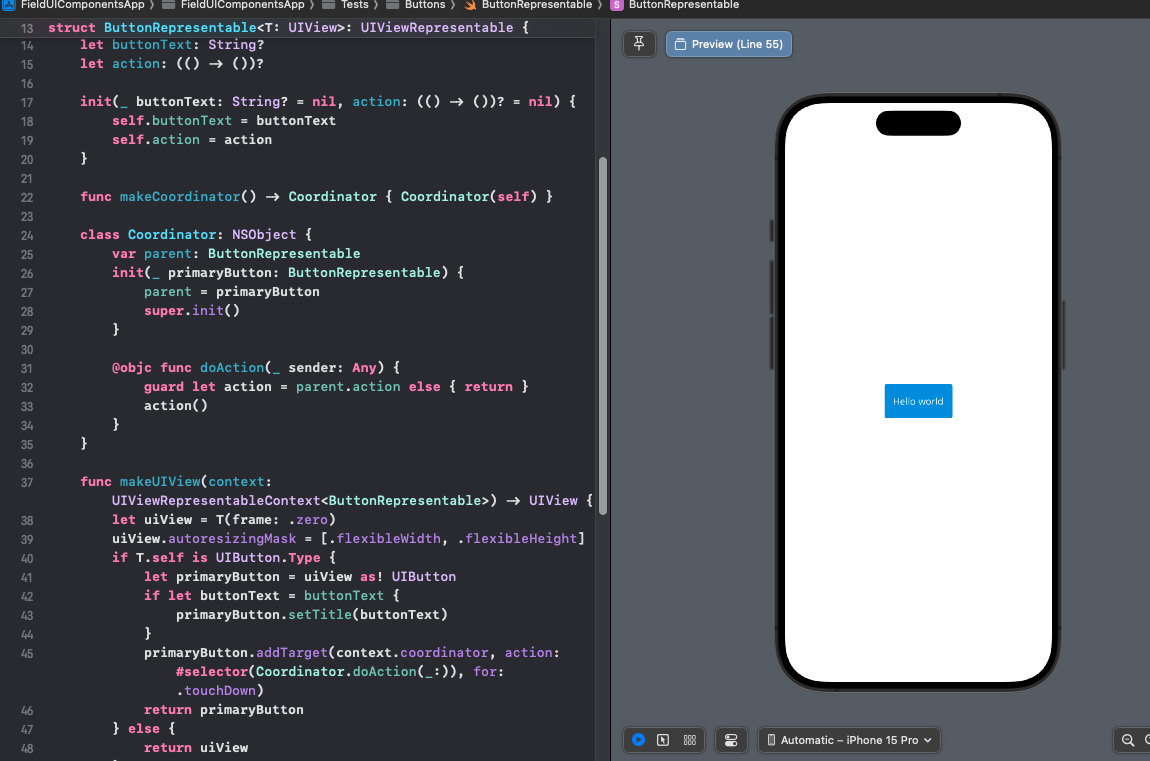
\includegraphics[width=1\textwidth]{Images/iOSButtonRepresentable.png}
    \caption{ButtonViewRepresentable failas}
    \label{fig:buttonViewRepresentable}
\end{figure}

\newpage
\subsubsection{Custom Toast message on Android}
Ši užduotis buvo skirta realizuoti UX sukurtą iššokančių žinučių (\emph{angl. Toast messages}) komponentą Android ir iOS operacinėse sistemose. 
Buvo sukurti FieldUIComponents app langai, kuriuose galima įvairiais būdais ištestuoti iššokančias žinutes.

Pasirinkau atlikti šią užduotį Android prietaisuose. 

Reikalavimai atliekant užduotį:
\begin{enumerate}
    \item Sukurti padengtą testais FieldUIComponents komponentą.
    \item Sukurti naują iššokančių žinučių komponentą.
    \begin{enumerate}
        \item Teksto žinutė
        \begin{enumerate}
            \item Tekstas turi tilpti į vieną eilutę.
            \item Jei tekstas užima daugiau vietos, sutrumpinti su \enquote{...}.
            \item Komponento animacija turi kiek galima daugiau sutapti su maketo animacijomis.
        \end{enumerate}
        \item Iššokančios žinutės animacijos trukmė - 3 sekundės.
        \item Iššokanti žinutė galima paslėpti paspaudus ant jos ar atlikus tempimo į viršų gestą.
    \end{enumerate}
    \item Iššokančių žinučių eilė:
    \begin{enumerate}
        \item Iššokančios žinutės patenka į eilę, rodomos viena po kitos, paslepiamos tokia pačia tvarka kaip ir buvo parodytos.
        \item Tokios pačios žinutės nerodomos 2 kartus.
    \end{enumerate}
\end{enumerate}
\bigskip
Iš pradžių buvo sukurtas iššokančios žinutės komponentas (\ref{fig:pill} paveikslėlis). Komponentui pritaikytos gestų atpažinimo, paspaudimo funkcionalumas, teksto sutrumpinimas (\ref{fig:pillCode} paveikslėlis).

\begin{figure}[htbp!]
    \centering
    \begin{minted}[linenos,tabsize=1,breaklines]{kotlin}
@Composable
fun Pill(
    modifier: Modifier = Modifier,
    text: String,
    fontSize: TextUnit = dimensionResource(id = R.dimen.toast_font_size).value.sp,
    horizontalPadding: Dp = dimensionResource(id = R.dimen.toast_padding_horizontal),
    verticalPadding: Dp = dimensionResource(id = R.dimen.toast_padding_vertical)
) {
    Surface(
        modifier = modifier
            .padding(horizontal = horizontalPadding),
        shape = CircleShape,
        color = colorResource(R.color.toastBackground)
    ) {
        Row(
            modifier = Modifier
                .wrapContentWidth()
                .padding(horizontalPadding, verticalPadding),
            horizontalArrangement = Arrangement.Center
        ) {
            Text(
                text = text,
                textAlign = TextAlign.Center,
                fontSize = fontSize,
                color = Color.White,
                style = MaterialTheme.typography.body2,
                maxLines = 1,
                overflow = TextOverflow.Ellipsis
            )
        }
    }
}
    \end{minted}
    \caption{Iššokančios žinutės komponento kodas}
    \label{fig:pillCode}
\end{figure}
\newpage
Sukurtas \enquote{ToastViewModel}, kuris rūpinasi iššokančių žinučių eile, patikrina eilėje esančias žinutes, jei eilėje egzistuoja žinutė, antrą kartą jos neparodys (\ref{fig:ToastViewModel} paveikslėlis). Taip pat galima pateikti žinutės trukmę. pasibaigus trukmei, žinutė išmetama iš eilės.

\begin{figure}[htbp!]
    \centering
    \begin{minted}[linenos,tabsize=1,breaklines]{kotlin}
class ToastViewModel : ViewModel() {
    private val _toastDataState = MutableStateFlow<ToastData?>(null)
    val toastDataState = _toastDataState.asStateFlow()

    private val mutex = Mutex()

    private var pendingMessages: MutableSet<String> = mutableSetOf()

    fun showToast(
        message: String,
        duration: Long = 3000L
    ) {
        if (pendingMessages.isEmpty() || pendingMessages.last() != message) {
            pendingMessages.add(message)
            viewModelScope.launchSafe {
                mutex.withLock {
                    try {
                        return@launchSafe suspendCancellableCoroutine { continuation ->
                            _toastDataState.value = ToastData(message, duration, continuation)
                        }
                    } finally {
                        _toastDataState.value = null
                        pendingMessages.remove(message)
                    }
                }
            }
        }
    }
}
    \end{minted}
    \caption{ToastViewModel programinis kodas}
    \label{fig:ToastViewModel}
\end{figure}

\newpage
Buvo sukurtas \enquote{ToastHost}, skirtas tvarkingai, su animacijomis parodyti iššokančias žinutes  (\ref{fig:ToastHost} paveikslėlis).

\begin{figure}[htbp!]
    \centering
    \begin{minted}[linenos,tabsize=1,breaklines]{kotlin}
...
val animationOffset: (Int) -> Int = { (heightToDropPx + it * 1.5).toInt() * -1 }
val springAnimationSpec: FiniteAnimationSpec<IntOffset> = spring(
    dampingRatio = Spring.DampingRatioMediumBouncy,
    stiffness = Spring.StiffnessMedium
)

LaunchedEffect(currentToastData) {
    setVisibility(true)
    delay(currentToastData.duration)
    setVisibility(false)
}

AnimatedVisibility(
    modifier = modifier.padding(top = heightToDrop),
    enter = slideInVertically(springAnimationSpec, initialOffsetY = animationOffset),
    exit = slideOutVertically(springAnimationSpec, targetOffsetY = animationOffset),
    visibleState = isVisible,
    content = { toast() }
)
...
    \end{minted}
    \caption{ToastHost programinis kodas}
    \label{fig:ToastHost}
\end{figure}

\newpage
Kadangi \enquote{Jetpack Compose} komponentų tiesiogiai integruoti į fragmentais pagrįstą programėlę, reikėjo sukurti papildomą klasę \enquote{Toasts} (\ref{fig:Toasts} paveikslėlis). Jame padavus tėvinį vaizdą (\emph{angl. root view}) programiniu būdu prideda \enquote{Jetpack Compose} komponentą. Galutinį rezultatą galima matyti \ref{fig:modelToastView} paveikslėlyje.

\begin{figure}[htbp!]
    \centering
    \begin{minted}[linenos,tabsize=1,breaklines]{kotlin}
class Toasts(private val context: Context) {
    private var view: View? = null
    fun addToastView(activityRootLayout: ViewGroup?) {
        val rootView = activityRootLayout ?: return
        if (view == null)
            createToastView(rootView)
    }

    private fun createToastView(rootView: ViewGroup) {
        val view = ComposeView(context).apply {
        setViewCompositionStrategy(ViewCompositionStrategy.DisposeOnViewTreeLifecycleDestroyed)
            setContent {
                Column {
                    Toast(toastViewModel = toastViewModel)
                }
            }
        }

        this.view = view
        rootView.addView(view)
        rootView.bringChildToFront(view)
        view.requestLayout()
    }
}
\end{minted}
    \caption{Toasts komponentas}
    \label{fig:Toasts}
\end{figure}